\subsection{Heuristic for Edge Perturbation}

The critical step of graph anonymization is to select a set of edges subject to modification. 
It needs to balances privacy gain and structural distortion. 
It involves consideration of the exponential number of edge combinations. 
Recently, the most popular paradigm for solving such problems has been using a class of heuristics. 
Successes of this approach include
(1) anonymity-aware ones that suggest injecting more considerable noise to unique nodes~\cite{Ying2009,Boldi_Injecting_2012,Hay_Anonymizing_2007} 
(2) utility-aware ones that indicate avoiding distortion over “bridge” edges whose deletion/addition would significantly impact the graph structure~\cite{Wang2011,Ninggal_Utility_2015}. 
The judicious edge selection must involve two types of heuristics which complement each other. 
Individually, they are far less effective. 
However, they have not been explored yet in the context of uncertain graphs.

Motived by the above, we first generalize the calibration of uniqueness with the marriage of KL-divergence function. 
Second, we propose a generalized version of edge relevance from an information-theoretic perspective.
Besides, we develop an efficient algorithm for its computation.
And, we show the use of such a criterion boosts edge selection efficiently and straightforwardly.

\textbf{Generalized Uniqueness}~~
The uniqueness criterion was used to measure how unique a given node is among all the nodes in the graph w.r.t a specific property. 
For a given node, its uniqueness score is the inverse of the commonness score of its property value $w$.
And, the commonness score of $w$ amounts to the weighted average distance among all other property values.

However, the conventional method merely formulates node properties as discrete values and relies on the geometric distance function to measure their distance.  
Thus, it fails to handle our problem where the property values are probabilistic.
In this work, we extend the preliminary version to handle the probabilistic case. 

\begin{figure}[!htb]
  \vspace{-2pt}
  \centering
        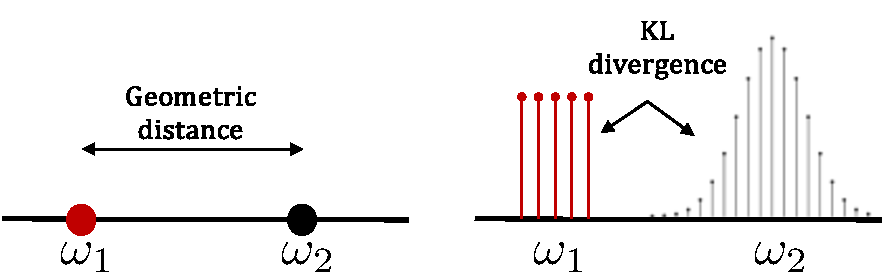
\includegraphics[width=\linewidth]{ill/shift_distance.pdf}
    \caption{The generalization of uniqueness.}
    \vspace{-10pt}
\end{figure}

We systematically model uncertain property values in both continuous and discrete domains as continuous and discrete random variables, respectively.
We consider the use of probability distributions, which are essential characteristics of uncertain property values, in the measuring similarity between uncertain property values. 
We use the well known Kullback-Leibler divergence to measure the distance between random variables with parameterized distributions. 
The generalized uniqueness can then be formalized as
\begin{definition}
    \textit{Uniqueness Score}
     Let $P:V \rightarrow  \Omega_{P}$ be a property on the set of nodes $V$ of the uncertain graph, 
     let $d$ be a KL divergence function, and let $\theta >0$  be a parameter. 
       Then the $\theta-$commonness of the property values $\omega$
       is $C_{\theta}(\omega):= \sum_{u \in V} \Phi_{0,\theta}(KL(\omega, P(v)))$,   
     while the corresponding uniqueness is $U_{\theta}:= \frac{1}{C_{\theta}(\omega)}$. 
     \vspace{-2pt}
\end{definition} 
Note that, the weights decays exponentially as a function of the KL divergence, 
and the parameter $\theta$ determines the decay rate. 
We set $\theta=\sigma$ as the injected noise blurs the meta-distribution of property values. 
 
\textbf{Generalized Edge Relevance}~~
It is clear that alteration over a single edge would produce local structural change and send ripples through the rest of the graph. 
The incurred structural distortion varies on the topological role of the edge subjecting to alteration, even with the same amount of modification. 
Targets at the high utility, we should penalize modification over structurally critical edges.  
It raised the need of measuring the relevance of edges in the uncertain graph. 


There are many potential ways to measure it. 
Importantly, the metric must fit the context of uncertain graphs.
Inspired by the importance of reliability, we measure the edge relevance of a given edge $e$ as the amount of structural distortion, measured by reliability discrepancy, caused by the unit noise subjects to the edge $e$, as follow. 
\begin{equation*}
  \begin{split}
    \mathcal{ERR}({e}) &= \frac{\Delta(\mathcal{G}+r_{e})}{|r_{e}|}  \\
                       &= \frac{\sum_{u,v} |R_{u,v}(\mathcal{G}+r_{e}) -R_{u,v}(\mathcal{G})|} {|r_{e}|}
  \end{split}
\end{equation*}

In the conventional case (deterministic graphs with edge addition and deletion $|r_{e}|=1$), it amounts to the connectivity structural distortion, measured by the number of connected node pairs.  
In probabilistic graphs, $\mathcal{ERR}$ is used to generalize this concept by quantifying the stochastic impact of partial edge addition/deletion over the connectivity of all the possible worlds.
It allows the estimation of structural distortion when $r_{e}$ lies in the contentious range. 

\begin{observation}
  Let $\mathcal{G}_{e}$, $\mathcal{G}_{\bar{e}}$ 
  denote two neighbor uncertain graphs $\mathcal{G}$ with $p(e)=1$ and $p(e)=0$ respectively. 
  The reliability relevance of an edge $e$ is a constant and equivalent to 
  the following function. 
  \begin{equation}
    \mathcal{ERR}(e) = \sum_{u,v} R_{u,v}(\mathcal{G}_{e}) \big- \sum_{u,v} R_{u,v}(\mathcal{G}_{\bar{e}})
    \label{eq:err}
  \end{equation}
  Observe that, the edge relevance only depends on it topological location. 
  It amounts to the difference of the number of connected pairs between two neighbor uncertain graphs. 
\end{observation}

\textbf{Proof Sketch.}~~
According to the possible world semantic and factorization rule, we can see that   
\begin{equation*}
  R_{u,v} (\mathcal{G}) = p(e) \cdot R_{u,v}(\mathcal{G}_{e}) ~+~ \big[ 1-p(e) \big] \cdot R_{u,v} (\mathcal{G}_{\bar{e}})
\end{equation*}
Note that, the two-terminal reliability $R_{u,v}$ in $\mathcal{G}_{e}$ and $\mathcal{G}_{\bar{e}}$ are constants. 
Therefore, two-terminal reliability discrepancy introduced by the single deviation $r_{e}$ over the uncertain graph $\mathcal{G}$ is equivalent to 
\begin{equation*}
  \begin{split}
    \Delta_{u,v} (\mathcal{G}+r_{e}) ~&= r_{e} \cdot R_{u,v}(\mathcal{G}_{e}) - r_{e} \cdot R_{u,v} (\mathcal{G}_{\bar{e}})\\
    &= r_{e} \cdot ~\big[  R_{u,v}(\mathcal{G}_{e}) - R_{u,v} (\mathcal{G}_{\bar{e}})  \big]
  \end{split}
\end{equation*}
Therefore, after aggregation and eliminating the factor $r_{e}$, the reliability relevance of an edge $e$ is equivalent to Equation~\ref{eq:err}. 

What is the relationship between Equation~\ref{eq:err} and the conventional cut-edge definition? 
In the deterministic scenario, a cut-edge is an edge of a graph whose deletion increase its number of connected components. 
One can quickly note that a cut-edge is a binary version of Equation~\ref{eq:err}, 
which is a continuous function regarding the edge deviation $r_{e}$ and reliability discrepancy. 
Therefore, $\mathcal{E}RR$ is not only relevant to connectivity discrepancy but also consider its scale.  

\textbf{Re-visiting the Computation Challenge}~~
\begin{figure}
  \vspace{-7pt}
    \subfigure[Iterative Evaluation]{\label{fig:itERR}
      \begin{minipage}[l]{0.46\columnwidth}
        \centering
        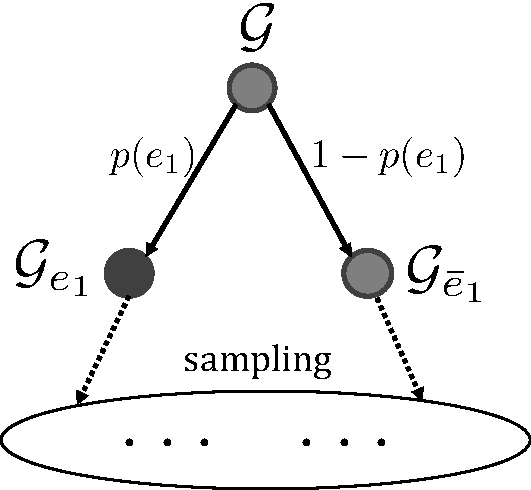
\includegraphics[height=2.7cm]{ill/iterativeERR.pdf}
      \end{minipage}
      }
    \subfigure[Memorized Evaluation]{\label{fig:groupERR}
      \begin{minipage}[l]{0.46\columnwidth}
        \centering
        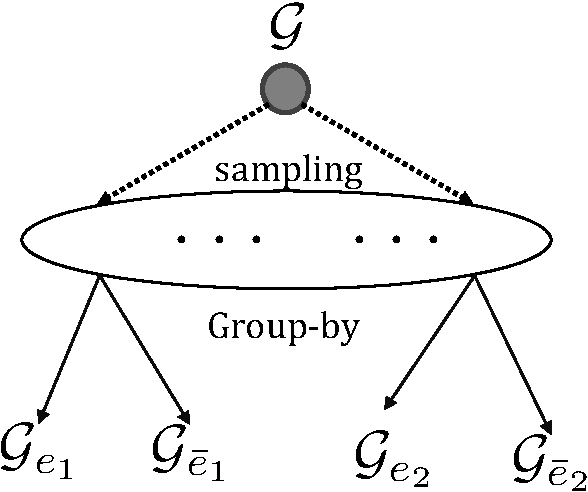
\includegraphics[height=2.7cm]{ill/groupERR.pdf}
      \end{minipage}
      }
    \vspace{-5pt}
    \caption{Sampling-based reliability detection}
    \label{fig:computationERR}
    \vspace{-7pt}
\end{figure} 
As ever mentioned, 
the evaluation of $\mathcal{E}RR(e)$ involves a fundamental problem concerning uncertain graphs, which we call 
the two-terminal reliability detection (TTR) problem. 
Since this problem is \#P-complete, we focus on efficiently and accurately approximate TTR.
The Monte-Carlo sampling method can be used to estimate the underlying reliability of an uncertain graph. 
Namely, we create a subset of possible worlds of the input uncertain graph with the use of edge sampling probabilities. 
Then, we take the average of the number of connected node pairs in the sampled worlds as an approximation. 
 
The $\mathcal{E}RR$ evaluation over all the edges is not trivial. 
One option is to iteratively invoke the sampling-based reliability computation over all the edges, 
as illustrated in Figure~\ref{fig:itERR}. 
It is straightforward to compute the connected components of a graph in linear time (regarding the numbers of the nodes and edges of the graph) using either breadth-first search or depth-first search.
For each edge, we need to perform the connected component detection for $N$ sampled graphs.
Thus, the overall time complexity is $\mathcal{O}(|E|\cdot N |E|)$.

Apparently, the baseline method is inefficient when the uncertain input graph is enormous.
XXXXX
Here, we present an efficient method which re-uses 
the connected components detection result of samples as illustrated in Figure~\ref{fig:groupERR}. 
For each edge $e$, we group the sampled possible worlds according to the edge existence, 
then get the average value of $cc$ over each group as accurate approximation of $cc(\mathcal{G}_{e})$ and $cc(\mathcal{G}_{\bar{e}})$.
The running time analysis roughly follows the analysis of the single-edge case.  
The overall time complexity is $\mathcal{O}(N |E|)$. 
By this way, we bring the evaluation of edge reliability relevance to the realm.